\documentclass[pra,12pt]{revtex4}
\usepackage{amsmath}
\usepackage{amssymb}
\usepackage{graphicx}
\usepackage{color}
\def\ket#1{\left|#1\right\rangle}
\def\bra#1{\left\langle#1\right|}
\def\braket#1{\left\langle#1\right\rangle}

\setlength{\parindent}{0pt}

\renewcommand{\baselinestretch}{1.0}
\setlength{\parskip}{0.07in}

\begin{document}

%% \section{Scattering Processes in Quantum Mechanics}

\section{Scattering experiments on quantum particles}

Quantum particles exhibit a feature known as \textbf{wave-particle
  duality}, which can be summarized using the following
\textbf{quantum double-slit thought experiment}.  As shown in the
figure, a source emits electrons with energy $E$, which move towards a
screen with a pair of slits.  A detector is positioned on the other
side of the screen.  By moving the detector around, we can measure the
rate at which electrons are detected at different positions.

\begin{figure}[h]
  \centering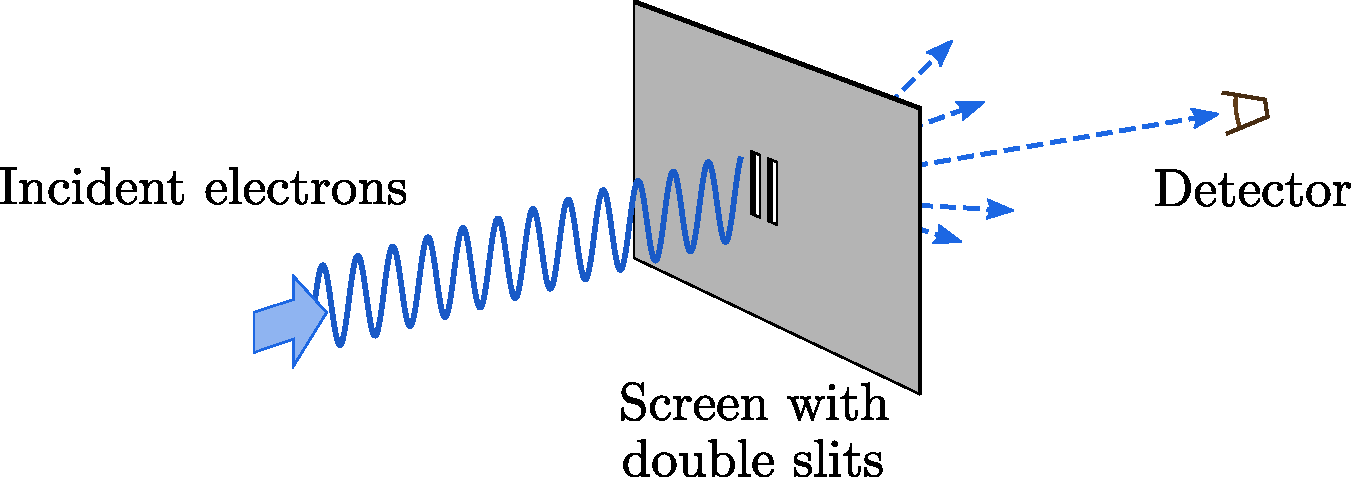
\includegraphics[width=0.6\textwidth]{doubleslit}
\end{figure}

According to quantum theory, the experiment will reveal the following:
(i) the detector finds electrons arriving in discrete units---one at a
time, like classical particles; (ii) when we move the detector around
to measure how the detection events are \textit{statistically}
distributed in space, the resulting distribution matches an
interference pattern formed by a classical wave diffracted by the
slits, with wavelength $\lambda$ related to the electron energy $E$ by
$$\lambda = \frac{2\pi}{k}, \;\;\; E = \frac{\hbar^2k^2}{2m},$$
where $\hbar = h/2\pi$ is Dirac's constant, and $m$ is the electron
mass.  Note, by the way, that if we assume the above relations hold,
then knowing the incident electron energy $E$, the diffraction pattern
can be used to deduce the spacing of the double slits.

Wave-particle duality arises from quantum theory's distinction between
a particle's state and the outcome of a measurement on it.  The state
is described by a wavefunction, $\psi(\mathbf{r})$, which can undergo
diffraction like a classical wave.  Measurement outcomes, however,
depend \textit{probabilistically} on the wavefunction; e.g., for a
position measurement, the probability of locating a particle in a
volume $dV$ around position $\mathbf{r}$ is $|\psi(\mathbf{r})|^2
\,dV$.

In this chapter, we will study a generalization of the quantum
double-slit experiment, called a \textbf{scattering experiment}.  The
idea is to take an object called a \textbf{scatterer}, shoot quantum
particles at it, and measure the resulting particle distribution.
Just as we can use the double-slit interference pattern to deduce the
spacing between the slits, a scattering experiment can likewise be
used to deduce various facts about the scatterer.  Scattering
experiments, as a class, constitute a large proportion of the methods
used to probe the quantum world---ranging from electron- and
photon-based laboratory experiments for measuring the properties of
materials, to huge accelerator experiments for probing high-energy
phenomena like the Higgs boson.

We will focus on a relatively simple scenario, consisting of a single
non-relativistic quantum particle and a classical scatterer.  Consider
a continuous and unbounded $d$-dimensional space, describable by
coordinates $\mathbf{r}$.  Somewhere around the origin, $\mathbf{r} =
0$, is a finite-sized scatterer.  An incoming quantum particle, with
energy $E$, is governed by the Hamiltonian
$$\hat{H} = \hat{H}_0 + V(\hat{\mathbf{r}}), \;\;\; \hat{H}_0 = \frac{\hat{\mathbf{p}}^2}{2m}.$$
Here, $\hat{H}_0$ describes the particle's kinetic energy, $m$ is the
particle's mass, $\hat{\mathbf{r}}$ and $\hat{\mathbf{p}}$ are
position and momentum operators, and $V$ is a \textbf{scattering
  potential} describing how the scatterer affects the quantum
particle.  We assume that $V(\mathbf{r}) \rightarrow 0$ as
$|\mathbf{r}| \rightarrow \infty$, i.e., the scattering potential
becomes negligible far from the origin.

\begin{figure}[h]
  \centering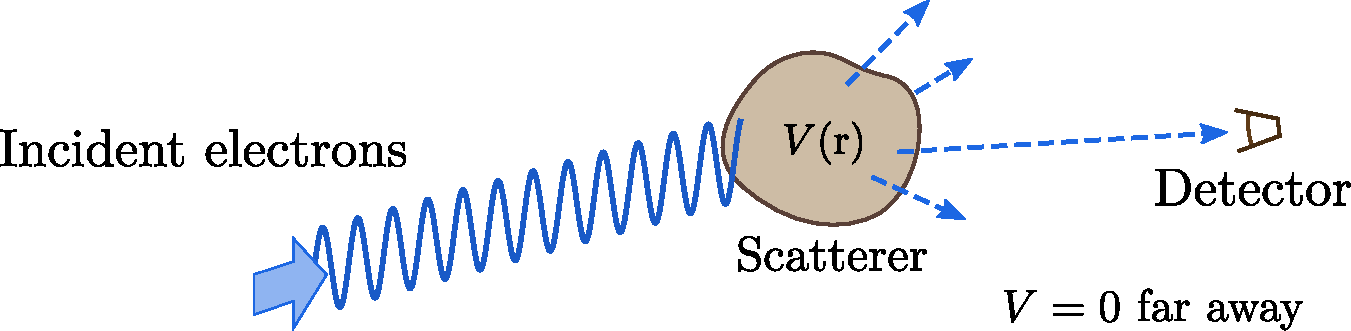
\includegraphics[width=0.6\textwidth]{scattering}
\end{figure}

We prepare an incoming particle state with energy $E$, and want to see
how the particle is scattered by the potential.  However, converting
these words into a well-defined mathematical problem is a bit tricky!
We will give the formulation first, before discussing its meaning:
\begin{enumerate}
\item 
The particle is described by a state $|\psi\rangle$ obeying the
time-independent Schr\"odinger equation
$$\hat{H} |\psi\rangle = E |\psi\rangle,$$
where $E$ is the incoming particle energy.  

\item
This state can be decomposed into two terms,
$$|\psi\rangle \,=\, |\psi_i\rangle \,+\, |\psi_s\rangle,$$
where $|\psi_i\rangle$ is called the \textbf{incident state} and
$|\psi_s\rangle$ is called the \textbf{scattered state}.  We will also
refer to $|\psi\rangle$ as the \textbf{total state}.

\item
The incident state is an eigenstate of $\hat{H}_0$ with energy $E$:
$$\hat{H}_0 |\psi_i\rangle = E |\psi_i\rangle.$$

\item
Lastly, we require the scattered state to be an ``outgoing'' state.
This is the most subtle requirement, and we will describe how to deal
with it later.
\end{enumerate}
The first of the above conditions says that the scattering process is
elastic; since the scatterer takes the form of a potential
$V(\mathbf{r})$, its interaction with the particle is conservative
(i.e., the total energy $E$ is fixed).  The second condition, when
viewed in the position basis, says that the particle's wavefunction
$\psi(\mathbf{r}) = \langle \mathbf{r} |\psi\rangle$ can be taken as a
superposition of an incoming wave and a scattered wave.  The third
condition says that far from the scatterer ($|\mathbf{r}|\rightarrow
\infty$), the incident wave has a fixed wavelength determined by the
energy $E$.  The final condition says that the scattered part of the
wavefunction must correspond to a wave moving out to infinity.

Given $|\psi_i\rangle$, $E$, and $V(\mathbf{r})$, we are to solve for
$|\psi_s\rangle$.  Note that \textit{this is not an eigenproblem}!
Usually, when dealing with the time-independent Schr\"odinger
equation, we treat it as an eigenproblem and solve for the energy
eigenvalues and eigenstates.  Here, however, $E$ is not an output of
the calculation, but part of the input---it describes the energy of
the incoming particles in the experiment.

\section{Recap: position and momentum states}

Before proceeding, let us review the properties of quantum particles
in free space.

In a $d$-dimensional space, a coordinate vector $\mathbf{r}$ is a real
vector of $d$ components.  A quantum particle can be described by the
position basis---a set of quantum states $\{|\mathbf{r}\rangle\}$, one
for each possible $\mathbf{r}$.  The $\mathbf{r}$'s form a continuum,
and so, like the real numbers, this set of states is uncountably
infinite.  If we are studying a particle trapped in a finite region
(e.g., a particle in a box), $\mathbf{r}$ is restricted to that
region; otherwise, $\mathbf{r}$ is any real $d$-dimensional vector.
In either case, $\{|\mathbf{r}\rangle\}$ spans the quantum
state space, so that the identity operator can be resolved as
$$\hat{I} = \int d^dr \, |\mathbf{r}\rangle \,\langle\mathbf{r}|,$$
where the integral is taken over all allowed $\mathbf{r}$.  It
follows that
$$\langle \mathbf{r} | \mathbf{r}' \rangle = \delta^d(\mathbf{r}-\mathbf{r}').$$
The position eigenstates are said to be ``delta-function normalized'',
rather than being normalized to unity, because the $\mathbf{r}$
vectors form a continuum rather than a discrete set.  In the above
equation, $\delta^d(\cdots)$ denotes the $d$-dimensional delta
function; for example, in 2D,
$$\langle x,y \,|\, x',y' \rangle = \delta(x-x') \, \delta(y-y').$$
The position operator $\hat{\mathbf{r}}$ can be defined by taking
$|\mathbf{r}\rangle$ and $\mathbf{r}$ as the eigenstates and
eigenvalues:
$$\hat{\mathbf{r}} |\mathbf{r}\rangle \,=\, \mathbf{r}\, |\mathbf{r}\rangle.$$

Momentum eigenstates can be constructed from position eigenstates via
Fourier transforms.  First, suppose that the allowed region of space
is a box of length $L$ on each side, and periodic boundary conditions
in every direction.  Define the set of wave-vectors $\mathbf{k}$
corresponding to plane waves that satisfy the periodic boundary
conditions at the boundaries of the box:
$$\Big\{\mathbf{k}  \; \Big| \; k_j = 2\pi m/L, \,m\in\mathbb{Z}, \;\text{for each} \; j = 1, \dots,d\, \Big\}.$$
Note that so long as $L$ is finite, the $\mathbf{k}$ vectors form a
discrete set.  Next, define
$$|\mathbf{k}\rangle = \frac{1}{L^{d/2}} \, \int d^dr \; e^{i\mathbf{k}\cdot\mathbf{r}} |\mathbf{r}\rangle,$$
where the integral is taken over the box.  These states
can be shown to satisfy the following:
$$\langle\mathbf{k}|\mathbf{k}'\rangle = \delta_{\mathbf{k},\mathbf{k}'}, \quad \langle\mathbf{r}|\mathbf{k}'\rangle = \frac{1}{L^{d/2}} e^{i\mathbf{k}\cdot\mathbf{r}}, \quad I = \sum_{\mathbf{k}} |\mathbf{k}\rangle\,\langle\mathbf{k}|.$$
The momentum operator is defined as an operator that has
$\{|\mathbf{k}\rangle\}$ as its eigenstates:
$$\hat{\mathbf{p}} |\mathbf{k}\rangle \,=\, \hbar \mathbf{k}\, |\mathbf{k}\rangle.$$
Thus, for finite $L$, the momentum eigenstates are discrete and
normalizable to unity; the momentum component in each direction is
quantized to a multiple of $\Delta p = 2\pi\hbar/L$.

Next, we take the limit of an infinite box, $L \rightarrow \infty$.
In this limit, $\Delta p \rightarrow 0$, and therefore the momentum
eigenvalues coalesce into a continuum.  In order to properly handle
the momentum eigenstates in this limit, it is conventional to alter
their normalization as follows:
$$|\mathbf{k}\rangle \rightarrow \left(\frac{L}{2\pi}\right)^{d/2} |\mathbf{k}\rangle.$$
Then, in the $L\rightarrow\infty$ limit, the re-normalized momentum
eigenstates satisfy
$$\boxed{\begin{aligned} |\mathbf{k}\rangle &= \frac{1}{(2\pi)^{d/2}} \, \int d^dr \; e^{i\mathbf{k}\cdot\mathbf{r}} |\mathbf{r}\rangle, \\ |\mathbf{r}\rangle &= \frac{1}{(2\pi)^{d/2}} \, \int d^dk \; e^{-i\mathbf{k}\cdot\mathbf{r}} |\mathbf{k}\rangle, \\\langle\mathbf{k}|\mathbf{k}'\rangle = \delta^d(\mathbf{k}-\mathbf{k}'),& \quad \langle\mathbf{r}|\mathbf{k}\rangle = \frac{1}{(2\pi)^{d/2}} e^{i\mathbf{k}\cdot\mathbf{r}}, \quad I = \int d^dk \;|\mathbf{k}\rangle\,\langle\mathbf{k}|,\end{aligned}}$$
with the integrals now taken over infinite spaces.  The position and
momentum eigenstates are now on a similar footing; in particular, both
are now delta-function normalized.  Note that in deriving the above
equations, it is helpful to use the formula
$$\int_{-\infty}^\infty dx\; \exp(ikx) \;=\; 2\pi\delta(k).$$

For an arbitrary quantum state $|\psi\rangle$, a wavefunction is
defined as the projection onto the position basis: $\psi(\mathbf{r}) =
\langle \mathbf{r}|\psi\rangle$.  Using the momentum eigenstates, we can
show that
$$\begin{aligned}\langle \mathbf{r}|\hat{\mathbf{p}}|\psi\rangle &=  \int d^dk \; \langle\mathbf{r}|\mathbf{k}\rangle \; \hbar\mathbf{k} \; \langle\mathbf{k}|\psi\rangle \\ &=  \int \frac{d^dk}{(2\pi)^{d/2}}\; \hbar\mathbf{k} \;e^{i\mathbf{k}\cdot\mathbf{r}} \langle\mathbf{k}|\psi\rangle \\ &=  -i\hbar\nabla \int \frac{d^dk}{(2\pi)^{d/2}}\; \;e^{i\mathbf{k}\cdot\mathbf{r}} \langle\mathbf{k}|\psi\rangle \\ &= -i\hbar \nabla\psi(\mathbf{r}).\end{aligned}$$
This result can also be used to prove Heisenberg's commutation relation
$[\hat{r}_i, \hat{p}_j] = i\hbar\delta_{ij}$.

\section{Scattering from a 1D delta-function potential}

We are now ready to solve our first scattering problem.  Consider a 1D
space with spatial coordinate denoted by $x$, and a scattering
potential that consists of a ``spike'' at $x = 0$:
$$V(x) = \frac{\hbar^2\gamma}{2m} \,\delta(x).$$
The form of the prefactor $\hbar^2\gamma/2m$ is chosen for later
convenience; the parameter $\gamma$, which has units of $[1/x]$,
controls the strength of the scattering potential.

\begin{figure}[h]
  \centering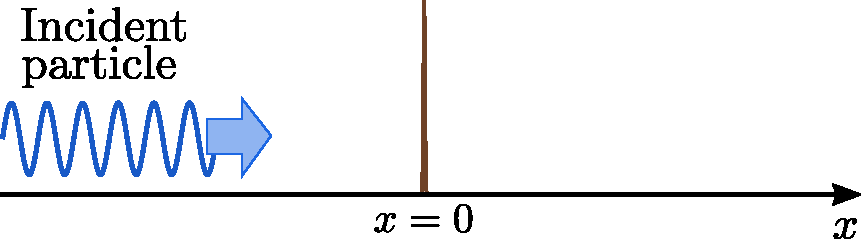
\includegraphics[width=0.45\textwidth]{scattering1d}
\end{figure}

You might be disturbed by the idea of a delta function potential, as
it is singular.  If so, just think of the delta function as a limiting
case of a family of non-singular functions (e.g., increasingly tall
and narrow gaussians centered at $x=0$).  When the Schr\"odinger wave
equation has a non-singular potential, any solution $\psi(x)$ must be
continuous and have well-defined first and second derivatives.  In the
delta function limit, the second derivative of $\psi(x)$ at $x=0$
blows up; moreover, the first derivative is discontinuous but finite,
while $\psi(x)$ itself remains continuous.  To verify this, integrate
the Schr\"odinger wave equation over an infinitesimal range around $x
= 0$:
$$\begin{aligned}\lim_{\varepsilon\rightarrow 0^+} \int_{-\varepsilon}^{+\varepsilon} dx\; \left[-\frac{\hbar^2}{2m} \frac{d^2}{dx^2} + \frac{\hbar^2\gamma}{2m} \delta(x)\right] \psi(x) &= \lim_{\varepsilon\rightarrow 0^+} \int_{-\varepsilon}^{+\varepsilon} dx\; E \psi(x) \\ = \lim_{\varepsilon\rightarrow 0^+} \left\{-\frac{\hbar^2}{2m} \left[\frac{d\psi}{dx}\right]_{-\varepsilon}^{+\varepsilon} \right\} + \frac{\hbar^2\gamma}{2m} \psi(0) &= 0\\ \Rightarrow \;\; \lim_{\varepsilon\rightarrow 0^+} \left\{\; \left.\frac{d\psi}{dx}\right|_{x = +\varepsilon} - \left.\frac{d\psi}{dx}\right|_{x = -\varepsilon}\; \right\}  &=  \gamma \,\psi(0).\end{aligned}$$

To proceed, consider a particle incident from the left, with energy
$E$.  This can be described by an incident state proportional to a
momentum eigenstate $|k_i\rangle$, where $k_i > 0$ and $E =
\hbar^2k_i^2/2m$.  We said ``proportional'', not ``equal'', as it is
conventional to normalize the incident state as follows:
$$|\psi_i\rangle = \sqrt{2\pi}\Psi_i |k_i\rangle \;\;\; \Leftrightarrow\;\;\; \psi_i(x) = \langle x|\psi\rangle = \Psi_i \, e^{ik_i x}.$$
The constant $\Psi_i$ is called the ``incident amplitude''; its
physical meaning will be discussed later.  Plug this into the
Schr\"odinger wave equation:
$$\left[-\frac{\hbar^2}{2m} \frac{d^2}{dx^2} + \frac{\hbar^2\gamma}{2m}\delta(x)\right] \left(\Psi_i \, e^{ikx} + \psi_s(x) \right) = E \left(\Psi_i \, e^{ikx} + \psi_s(x) \right)$$
Taking $E = \hbar^2k_i^2/2m$, and doing a bit of algebra, simplifies this to
$$\left[ \frac{d^2}{dx^2} + k_i^2\right] \psi_s(x) =  \gamma \delta(x) \left(\Psi_i \, e^{ikx} + \psi_s(x) \right).$$
This has the form of an inhomogenous ordinary differential equation (ODE)
for $\psi_s(x)$, with the potential term on the right acting
as a ``driving term''.  To find the solution, consider the two regions $x <
0$ and $x > 0$.  Since $\delta(x) \rightarrow 0$ for $x \ne 0$, the
equation in each half-space reduces to
$$\left[\frac{d^2}{dx^2} + k_i^2\right] \psi_s(x) = 0.$$
This second-order ODE is called the \textbf{Helmholtz equation}.  Its
general solution can be written as
$$\psi_s(x) = \Psi_i \left(f_1 e^{ik_i x} + f_2 e^{-ik_i x}\right),$$
where $f_1$ and $f_2$ are arbitrary complex constants.  These
constants can have different values in the two regions $x < 0$ and $x
> 0$.

We want $\psi_s(x)$ to describe an \textbf{outgoing wave}, moving away
from the scatterer towards infinity.  So, it should be purely
left-moving for $x < 0$, and purely right-moving for $x > 0$.  To
achieve this, we let $f_1 = 0$ for $x < 0$, and $f_2 = 0$ for $x > 0$,
so that $\psi_s(x)$ has the form
$$\psi_s(x) = \Psi_i \times \begin{cases}f_- \,e^{-ik_ix}, & x < 0 \\ f_+ \,e^{ik_ix}, & x > 0.\end{cases}$$
The complex numbers $f_-$ and $f_+$ are called \textbf{scattering
  amplitudes}.  They describe the magnitude and phase of the
wavefunction scattered backwards into the $x<0$ region, and scattered
forward into the $x > 0$ region, respectively.

To calculate the scattering amplitudes, we first recall from earlier
that the total wavefunction $\psi(x)$ must be continuous everywhere,
including at $x = 0$.  Since $\psi_i(x)$ is continuous, $\psi_s(x)$
must be as well, which means that $f_- = f_+$.

Moreover, we previously found that the first derivative of $\psi(x)$
is discontinuous at $x=0$:
$$\lim_{\varepsilon\rightarrow 0^+} \left\{\; \left.\frac{d\psi}{dx}\right|_{x = +\varepsilon} - \left.\frac{d\psi}{dx}\right|_{x = -\varepsilon}\; \right\}  =  \gamma\, \psi(0).$$
Plugging in our expression for $\psi(x)$ gives
$$\begin{aligned}\Psi_i\left[ik_i(1+f_\pm) - ik_i(1-f_\pm)\right]  &=  \Psi_i(1+f_\pm) \gamma \\ \Rightarrow \;\;\; f_+ = f_- = -\frac{\gamma}{\gamma - 2ik_i}.\end{aligned}$$

For now, let us focus on the magnitude of the scattering amplitude (we
will see, in the next chapter, that the phase also contains
interesting an useful information).  The quantity $|f_\pm|^2$
describes the overall strength of the scattering process:
$$|f_\pm|^2 = \left[1 + \frac{8mE}{(\hbar\gamma)^2}\right]^{-1}.$$

\begin{figure}[h]
  \centering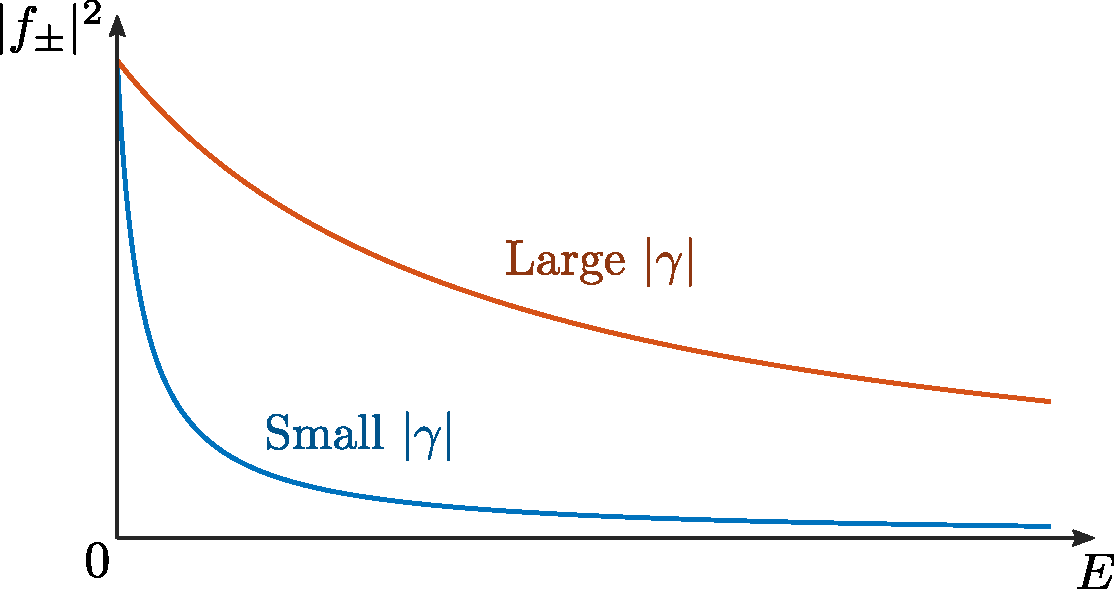
\includegraphics[width=0.55\textwidth]{scattering1df}
\end{figure}

The result is plotted above.  It has a number of notable features.
First, for a fixed potential strength $\gamma$, the scattering
strength decreases monotonically with $E$; i.e., higher-energy
particles are scattered less easily, which makes sense.  Second, for
given $E$, the scattering strength increases with $|\gamma|$, with the
limit $|f|^2 \rightarrow 1$ as $|\gamma|\rightarrow \infty$.  Third,
an attractive potential ($\gamma < 0$) and a repulsive potential
($\gamma > 0$) are equally effective at scattering the particle.

\section{Scattering in 2D and 3D}

We now consider scattering experiments in spatial dimension $d \ge 2$.
Compared to the 1D example discussed in the previous section, these
cases have an important distinguishing feature.  For $d = 1$, the
particle can only scatter forward or backward, but for $d \ge 2$ it
can also scatter ``sideways''.  The concept of an outgoing
wavefunction must therefore be formulated with care.

Far from the scatterer, where $V(\mathbf{r})\rightarrow 0$, we know
that the scattered wavefunction $\psi_s(\mathbf{r})$ satisfies the
free-space Schr\"odinger wave equation:
$$-\frac{\hbar^2}{2m} \nabla^2 \psi_s(\mathbf{r}) = E \psi_s(\mathbf{r}).$$
Here, $\nabla^2$ denotes the $d$-dimensional Laplacian.  Let $E =
\hbar^2 k^2 / 2m$, where $k \in \mathbf{R}^+$ is the wavenumber in
free space.  Then the above equation can be written as
$$\left[\nabla^2 + k^2\right] \psi_s(\mathbf{r}) = 0,$$
which is the Helmholtz equation in $d$-dimensional space.

One set of elementary solutions to the Helmholtz equation are the
plane waves, $\exp(i\mathbf{k}\cdot\mathbf{r})$, where $|\mathbf{k}| =
k$.  But we're looking for an outgoing solution, and a plane wave
can't be said to be ``outgoing'' (or ``incoming'').  To find such a
solution, we turn to curvilinear coordinates.

In 2D, we can adopt polar coordinates $(r,\phi)$, and look for
separable solutions to the Helmholtz equation of the form
$A(r)B(\phi)$.  Skipping the math details, the result is that the
general solution to the 2D Helmholtz equation can be written as
$$\psi(\mathbf{r})=\sum_{\pm}\sum_{m=-\infty}^\infty c_m^\pm\,H_m^\pm(kr)\,e^{im\phi}.$$
Each $c_m^\pm$ is a complex coefficient, and $H_m^\pm$ is a special
function called a \textbf{Hankel function} of the first kind ($+$) or second
kind ($-$).  Each term in the sum describes a wave component that has a
definite angular momentum, and is moving either toward or away from the
origin.  The integer index $m$ specifies the angular momentum, while
$\pm$ denotes whether it is outgoing ($+$) or incoming ($-$); this is
because, far from the origin, the Hankel functions reduce to
$$H_m^\pm(kr) \overset{r\rightarrow\infty}{\longrightarrow} \sqrt{\frac{2}{\pi kr}} \, \exp\left[\pm i\left(kr - \frac{(m+\frac{1}{2})\pi}{2}\right)\right] \;\sim\; r^{-1/2} e^{ikr}.$$

\textcolor{red}{[Fig.]}

In 3D, we use spherical coordinates $(r,\theta,\phi)$.  Again skipping
the math details, the general solution to the Helmholtz equation can
be written as
$$\psi(\mathbf{r})=\sum_{\pm}\sum_{l=0}^\infty\sum_{m=-l}^lc_{lm}^\pm\,h_l^\pm(kr)\,Y_{lm}(\theta,\phi).$$
The $c$'s are again complex coefficients, each $h_l^\pm$ is a
\textbf{spherical Hankel function}, and each $Y_{lm}$ is a
\textbf{spherical harmonic}.  The $l$ and $m$ indices specify the
angular momentum of each wave component, while $\pm$ denotes if it is
outgoing ($+$) or incoming ($-$); far from the origin,
$$h_l^\pm(kr) \overset{r\rightarrow\infty}{\longrightarrow} \frac{1}{kr}\,\exp\left[\pm i\left(kr-\frac{(l+1)\pi}{2}\right)\right] \;\sim\; r^{-1} e^{ikr}.$$

It is now clear what we need to do to get a scattered wavefunction
$\psi_s(\mathbf{r})$ that is outgoing at infinity.  We take the
general solution and discard all incoming ($-$) wave components,
keeping only the $+$ terms:
$$\psi_s(\mathbf{r}) = \begin{cases} \displaystyle\sum_{m} c_m^+\,H_m^\pm(kr)\,e^{im\phi}, &d=2\\ \displaystyle\sum_{lm} c_{lm}^+\,h_l^+(kr)\,Y_{lm}(\theta,\phi),&d=3.\end{cases}$$
For large $r$, the outgoing wavefunction's $r$-dependence can be
written as
$$\psi_s(\mathbf{r}) \; \overset{r\rightarrow\infty}{\sim} \; r^{\frac{1-d}{2}} e^{ikr}.$$

For $d > 1$, the magnitude of the wavefunction decreases with distance
from the origin.  This is to be expected, because with increasing $r$,
an outgoing wave spreads out over a wider area.  To verify this
intuition, consider the probability current density
$\mathbf{J} = (\hbar/m) \mathrm{Im}\left[\psi_s^*\nabla\psi_s\right]$;
its $r$-component is
$$\begin{aligned}J_r \; &\overset{r\rightarrow\infty}{\sim} \; \mathrm{Im}\left[r^{\frac{1-d}{2}} e^{-ikr} \frac{\partial}{\partial r}\left(r^{\frac{1-d}{2}} e^{ikr}\right)\right] \\ &\;\;=\;\;\;\mathrm{Im}\left[\frac{1-d}{2}\, r^{-d} + ik r^{1-d}\right]\\ &\;\;=\;\;\; kr^{1-d}.\end{aligned}$$
In $d$ dimensions, the ``area'' of a ``spherical'' wave-front scales
as $r^{d-1}$, so the probability flux goes as $J_r \,r^{d-1} \sim k$,
independent of $r$.  Thus, the outgoing solution describes a constant
probability flux flowing outward from the origin.  Note also that if
we plug $d=1$ into the above formula, we get a scattered probability
flux that scales as $r^0$ (i.e., a constant), which is consistent
with the findings from the 1D model in the previous section.
In 1D, waves do not spread out with distance since there is no
transverse dimension; accordingly, $\psi_s$ and $J_r$ are independent
of the distance traveled.

\section{The scattering amplitude and scattering cross section}

We can use the results of the previous section to systematically
characterize the outcomes of a scattering experiment.  Let the
incident wavefunction be a plane wave,
$$\psi_i(\mathbf{r}) = \Psi_i \, e^{i\mathbf{k}_i\cdot\mathbf{r}},$$
in $d$-dimensional space.  Here, $\Psi_i \in \mathbb{C}$ is the
\textbf{incident wave amplitude}, and $\mathbf{k}_i$ is the incident
momentum.  We let $k_i = |\mathbf{k}_i|$ denote its magnitude, so that
the particle energy is $E = \hbar^2k_i^2/2m$.  We adopt coordinates
$(r,\Omega)$, where $r$ is the distance from the origin.  For 1D,
$\Omega \in \pm$ which specifies the choice of ``forward'' or
``backward'' scattering; for 2D polar coordinates, $\Omega = \phi$;
and for 3D spherical coordinates, $\Omega = (\theta,\phi)$.  According
to the previous section, the scattered wavefunction reduces to the
following form far from the origin:
$$\psi_s(\mathbf{r})\;  \overset{r\rightarrow\infty}{\longrightarrow}\; \Psi_i \, r^{\frac{1-d}{2}} \, e^{ik_ir} \, f(\Omega).$$
The complex function $f(\Omega)$, called the \textbf{scattering
  amplitude}, is the fundamental object of interest in scattering
experiments.  It describes how the particle is scattered in various
directions, and it depends on the inputs to the scattering problem,
including $\mathbf{k}_i$ and the scattering potential.  From it, we
can also define two other important quantities of interest:
$$\boxed{\begin{aligned}\frac{d\sigma}{d\Omega} &= \big|f(\Omega)\big|^2 \qquad\quad\quad \text{(the \textbf{differential scattering cross section})} \\ \sigma &= \int d\Omega\; \big|f(\Omega)\big|^2 \quad\; \text{(the \textbf{total scattering cross section}).}
  \end{aligned}}$$
In the second equation, $\int d\Omega$ denotes the integral(s) over
all the angle coordinates (or, in 1D, a sum over the two directions
$\Omega \in \pm$).

The term ``cross section'' comes from an analogy with the scattering
of classical particles.  To understand this, consider the probablity
current density associated with the scattered wavefunction:
$$\mathbf{J}_s = \frac{\hbar}{m} \mathrm{Im}\big[\psi_s^*\nabla\psi_s\big].$$
Let us focus only on the $r$-component of the current density, in the
$r\rightarrow\infty$ limit:
$$\begin{aligned}J_{s,r}\; &\;\;=\;\;\;\, \frac{\hbar}{m}\, \mathrm{Im}\left[\psi_s^* \frac{\partial}{\partial r}\psi_s\right] \\ &\overset{r\rightarrow\infty}{\longrightarrow}\;\, \frac{\hbar}{m}\; |\Psi_i|^2 \; |f(\Omega)|^2 \mathrm{Im}\left[\left(r^{\frac{1-d}{2}} \, e^{ik_ir}\right)^* \frac{\partial}{\partial r} \left(r^{\frac{1-d}{2}} \, e^{ik_ir}\right)\right] \\ & \;\;=\;\;\;\, \frac{\hbar \,k_i}{m}\; |\Psi_i|^2 \; |f(\Omega)|^2 \,r^{1-d}.\end{aligned}$$
The total flux of outgoing probability is obtained by integrating
$J_{s,r}$ over a constant-$r$ surface:
$$I_s \;=\; \int d\Omega\; r^{d-1} \, J_{s,r} \;=\; \frac{\hbar k_i}{m} \;|\Psi_i|^2 \; \int d\Omega\; \big|f(\Omega)\big|^2.$$
We can assign a physical interpretation to each term in this
result.  The first factor, $\hbar k_i/m$, is the
particle's speed (i.e., the group velocity of the de Broglie wave).
The second factor, $|\Psi_i|^2$, is the probability density of the incident
wave, which has units of $[x^{-d}]$ (i.e., inverse $d$-dimensional
``volume'').  The product of these two factors represents the
\textbf{incident flux},
$$J_{i} = \frac{\hbar k_i}{m} \;|\Psi_i|^2.$$
This has units of $[x^{1-d}t^{-1}]$ (i.e., rate per unit ``area'').

Now, let us re-imagine this incident flux $J_i$ as a stream of
classical particles, and the scatterer as a ``hard-body'' scatterer
that only interacts with those particles striking it directly.  The
scattering rate will be $J_{i}$ times the cross-sectional area of the
scatterer exposed to the particle stream.  If we denote this area by
$\sigma$, the scattering rate is
$$I_s = J_i \, \sigma.$$

\begin{figure}[h]
  \centering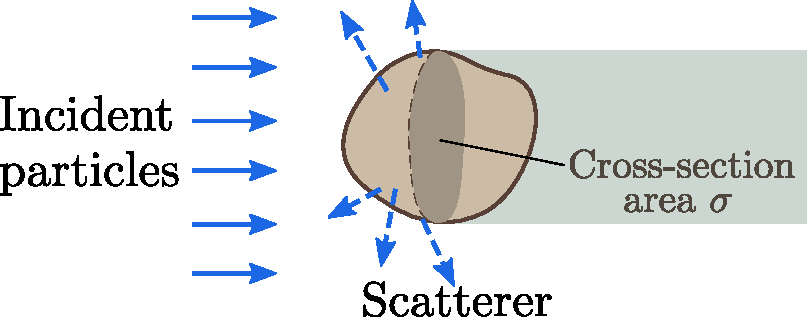
\includegraphics[width=0.5\textwidth]{crosssection}
\end{figure}

Comparing this to the quantum scattering expression, we identify $\int
d\Omega\,|f|^2$ as playing a role analogous to the classical hard-body
cross-sectional area.  We hence call this the ``total scattering cross
section''.  Moreover, this quantity is expressed as an integral over
angles; the integrand $|f|^2$ is called the ``differential scattering
cross section'', and it represents the rate, per unit of solid angle,
at which particles are scattered in a given direction.

\section{The Green's function}

Having defined the scattering amplitude $f(\Omega)$, we still need to
figure out how to calculate it.  This can be done using a variety of
methods, including numerical methods.  We will focus on one
particularly important approach, which is a quantum mechanical version
of the classical Green's function technique for solving inhomogenous
differential equations.

Let us return to the previously-discussed formulation of the
scattering problem:
$$\begin{aligned} \hat{H} &= \hat{H}_0+\hat{V}, \,\,\quad\quad |\psi\rangle = |\psi_i\rangle \,+\, |\psi_s\rangle, \\ \hat{H} |\psi\rangle &= E |\psi\rangle, \quad\quad \hat{H}_0 |\psi_i\rangle = E |\psi_i\rangle.\end{aligned}$$
These equations can be combined as follows:
$$\begin{aligned} \left(\hat{H}_0 + \hat{V}\right) |\psi_i\rangle + \hat{H} |\psi_s\rangle &= E \left( |\psi_i\rangle + |\psi_s\rangle \right) \\ \Rightarrow \quad \hat{V} |\psi_i\rangle + \hat{H} |\psi_s\rangle &= E |\psi_s\rangle  \\ \Rightarrow \quad\; \left(E - \hat{H}\right) |\psi_s\rangle & = \hat{V} |\psi_i\rangle
\end{aligned}$$
To proceed, we define the inverse of the operator on the left-hand
side:
$$\hat{G} = \big(E-\hat{H}\big)^{-1}.$$
This operator is called the \textbf{Green's function}.  Using it, we
get
$$|\psi_s\rangle = \hat{G} \hat{V} |\psi_i\rangle.$$

Note that $\hat{G}$ is dependent on both the energy $E$ and the
scattering potential.  To help isolate the dependence on the
scattering potential, let us define
$$\hat{G}_0=\big(E-\hat{H}_0\big)^{-1},$$
which is the Green's function for a free particle.  This will be very
useful for us, because $\hat{G}_0$ can be calculated exactly (as we
shall see in the next section), whereas $\hat{G}$ typically has no
finite exact expression.  We can relate $G$ to $G_0$ as follows:
$$\begin{aligned}\hat{G}(E-\hat{H}_0 - \hat{V})\;\; &= I \;\;\;\mathrm{and}\;\; (E-\hat{H}_0 - \hat{V})\hat{G} = I \\ \Rightarrow \;\;\; \hat{G} \hat{G}_0^{-1} - \hat{G}\hat{V} &= I \;\;\; \mathrm{and}\;\; \hat{G}_0^{-1} \hat{G} - \hat{V}\hat{G} \;\;\;= I\end{aligned}$$
Upon respectively right-multiplying and left-multiplying these equations
by $\hat{G}_0$, we arrive at the following pair of equations, called
\textbf{Dyson's equations}:
$$\boxed{\begin{aligned} \;\;\hat{G} \;&= \; \hat{G}_0 + \hat{G}\hat{V}\hat{G}_0\;\; \\ \;\;\hat{G} \;&=\; \hat{G}_0 + \hat{G}_0\hat{V}\hat{G} \;\;\end{aligned}}$$
These two equations are ``implicit'' equations, since the unknown
quantity we're interested in, $\hat{G}$, appears in both the left and
right sides.  Applying the second of Dyson's equation to the
scattering problem gives
$$\begin{aligned}|\psi_s\rangle &= \left(\hat{G}_0 + \hat{G}_0\hat{V}\hat{G}\right) \hat{V} |\psi_i\rangle \\ &= \hat{G}_0 \hat{V} |\psi_i\rangle + \hat{G}_0\hat{V}\hat{G} \hat{V} |\psi_i\rangle \\ &= \hat{G}_0 \hat{V} |\psi_i\rangle + \hat{G}_0\hat{V} |\psi_s\rangle \\ &= \hat{G}_0\hat{V} |\psi\rangle.\end{aligned}$$
This is a useful simplification, since it involves $\hat{G}_0$ rather
than $\hat{G}$.  The downside is that the equation is implicit, since
the right-hand side contains not $|\psi_i\rangle$ (which is given to
us), but the total state $|\psi\rangle$ (which we do not know).

One way we can try to solve the implicit equation is to plug the
expression for $|\psi_s\rangle$ repeatedly back into the right-hand
side.  This yields an infinite series formula:
$$\begin{aligned}|\psi_s\rangle &= \hat{G}_0 \hat{V} \left(|\psi_i\rangle + \hat{G}_0 \hat{V}|\psi\rangle\right) \\ &= \quad \vdots \\ &= \left[\hat{G}_0 \hat{V} + (\hat{G}_0 \hat{V})^2 + (\hat{G}_0 \hat{V})^3 + \cdots\right]|\psi_i\rangle.\end{aligned}$$
Or, equivalently,
$$|\psi\rangle = \left[\hat{I} + \hat{G}_0 \hat{V} + (\hat{G}_0 \hat{V})^2 + (\hat{G}_0 \hat{V})^3 + \cdots\right]|\psi_i\rangle.$$
This is called the \textbf{Born series}.  To understand its meaning,
let us go to the position basis:
$$\begin{aligned}\psi(\mathbf{r}) = \psi_i(\mathbf{r}) &+ \int d^dr' \langle \mathbf{r} | \hat{G}_0 |\mathbf{r}'\rangle\, V(\mathbf{r}') \psi_i(\mathbf{r}') \\ &+ \int d^dr' d^dr'' \langle \mathbf{r} | \hat{G}_0 |\mathbf{r}'\rangle\, V(\mathbf{r}') \, \langle \mathbf{r} | \hat{G}_0 |\mathbf{r}'\rangle \, V(\mathbf{r}'') \psi_i(\mathbf{r}'') \\ &+ \;\;\cdots\end{aligned}$$
The Born series describes the phenomenon of \textbf{multiple
  scattering}.  As a result of the presence of the scatterer, the
particle wavefunction consists of a quantum superposition of
wavefunctions with zero, one, two, or more scattering events.  For
example, the second-order term is
$$\int d^dr' d^dr'' \langle \mathbf{r} | \hat{G}_0 |\mathbf{r}'\rangle\, V(\mathbf{r}') \, \langle \mathbf{r} | \hat{G}_0 |\mathbf{r}'\rangle \, V(\mathbf{r}'') \psi_i(\mathbf{r}'')$$
which describes the particle undergoing the following process: (i)
scattering of the incident particle at point $\mathbf{r}''$, (ii)
propagation from $\mathbf{r}''$ to $\mathbf{r}'$, (iii) scattering
again at point $\mathbf{r}'$, and (iv) propagation from $\mathbf{r}'$
to $\mathbf{r}$.  The scattering points $\mathbf{r}'$ and
$\mathbf{r}''$ are integrated over, with all possible positions
contributing to the result; since the integrals are weighted by $V$,
those positions where the scattering potential are strongest will
contribute the most.

\textcolor{red}{[Fig.]}

Each successive term in the Born series involves more scattering
events, i.e.~more multiples of the scattering potential $\hat{V}$.
Hence, for a sufficiently weak scatterer it should be a good
approximation to retain just the first few terms.  For the rest of
this discussion, let us assume that such an approximation is valid.
(The question of what it means for $\hat{V}$ to be
``sufficiently weak''---i.e., the exact requirements for the Born
series to converge---is a complex topic that is beyond the scope of
our present discussion.)

\section{The Green's function for a free particle}
  
We have defined the free-particle Green's function as the operator
$$\hat{G}_0=\big(E-\hat{H}_0\big)^{-1}.$$
Its matrix element in the position basis,
$\langle\mathbf{r}|\hat{G}_0|\mathbf{r}'\rangle$, is called the
\textbf{propagator}.  As we have just seen, when the Born series is
written in the position basis, the propagator appears in the integrand
and describes how the particle travels, or ``propagates'', between
scattering points.

We can calculate the propagator with the aid of the momentum
eigenstates:
$$\begin{aligned}\langle\mathbf{r}|\hat{G}_0|\mathbf{r}'\rangle &=
  \langle\mathbf{r}|\hat{G}_0 \Big(\int d^dk |\mathbf{k}\rangle\langle\mathbf{k}| \Big) |\mathbf{r}'\rangle \\ &= \int d^dk \; \langle\mathbf{r}|\mathbf{k}\rangle \; \frac{1}{E-\frac{\hbar^2|\mathbf{k}|^2}{2m}} \; \langle\mathbf{k}|\mathbf{r}'\rangle \\ &= \frac{2m}{\hbar^2} \frac{1}{(2\pi)^d} \int d^dk \; \frac{\exp\left[i\mathbf{k}\cdot (\mathbf{r}-\mathbf{r}')\right]}{k_i^2-|\mathbf{k}|^2},\end{aligned}$$
where $k_i$ is the free-space wavenumber, related to the
particle energy by $E = \hbar^2 k_i^2/2m$.

To proceed, it is necessary to pick a value for the spatial dimension $d$.  We
will show the $d = 3$ case (the calculations for other $d$ are fairly
similar).  To calculate the three-dimensional integral over $k$-space,
we adopt spherical coordinates, denoted by $(k,\theta,\phi)$.  The
axes of the spherical coordinates are aligned so that $\theta$ is the
angle between $\mathbf{r}$ and $\mathbf{r}'$.  We can now do the $k$-space
integral:
$$\begin{aligned}\langle\mathbf{r}|\hat{G}_0|\mathbf{r}'\rangle &= \frac{2m}{\hbar^2} \frac{1}{(2\pi)^3} \int d^3k \; \frac{\exp\left[i\mathbf{k}\cdot (\mathbf{r}-\mathbf{r}')\right]}{k_i^2-|\mathbf{k}|^2} \\ &= \frac{2m}{\hbar^2} \frac{1}{(2\pi)^3} \int_0^\infty dk \int_0^\pi d\theta \int_{0}^{2\pi} d\phi \;k^2\sin\theta\; \frac{\displaystyle \exp\left(ik|\mathbf{r}-\mathbf{r}'|\cos\theta\right)}{k_i^2-k^2} \\ &= \frac{2m}{\hbar^2} \frac{1}{(2\pi)^2} \int_0^\infty dk \int_{-1}^1 d\mu \;k^2\; \frac{\displaystyle \exp\left(ik|\mathbf{r}-\mathbf{r}'|\mu\right)}{k_i^2-k^2} \qquad(\text{letting}\;\mu = \cos\theta) \\ &= \frac{2m}{\hbar^2} \frac{1}{(2\pi)^2} \int_0^\infty dk \; \frac{ k^2}{k_i^2-k^2}\, \frac{\displaystyle \exp\left(ik|\mathbf{r}-\mathbf{r}'|\right) - \exp\left(-ik|\mathbf{r}-\mathbf{r}'|\right)}{ik|\mathbf{r}-\mathbf{r}'|} \\ &= \frac{2m}{\hbar^2} \frac{1}{(2\pi)^2} \frac{i}{|\mathbf{r}-\mathbf{r}'|} \int_{-\infty}^\infty dk \; \frac{\displaystyle k\, \exp\left(ik|\mathbf{r}-\mathbf{r}'|\right)}{(k - k_i)(k+k_i)}\end{aligned}$$
The remaining integral looks like something we can do using contour
integration techniques.  But there's a snag: the integration contour
runs over the real-$k$ line, and since $k_i \in \mathbb{R}^+$, there
are two poles on the contour (at $\pm k_i$).  Hence, the value of the
integral, as written, is formally singular.

To give the integral a well-defined value, we must ``regularize'' it
by somehow tweaking its definition.  One way is to displace the poles
infinitesimally in the complex-$k$ plane, shifting them off the
contour.  We have a choice of whether to move each pole upwards or
downwards, and this choice turns out to be linked to whether the
Green's function describes waves that are incoming or out-going (or
behave in some other way) at infinity.  For us, it turns out that the
right choice is to move the pole at $-k_i$ infinitesimally downwards,
and move the pole at $+k_i$ infinitesimally upwards:

\textcolor{red}{[Fig.]}

This means replacing the denominator of the integrand as
follows:
$$(k - k_i)(k+k_i) \;\rightarrow\; (k - k_i - i\varepsilon)(k+k_i+i\varepsilon) = k^2 - (k_i+i\varepsilon)^2,$$
where $\varepsilon$ is a positive infinitesimal.  This is equivalent
to replacing $E \rightarrow E + i\varepsilon$ in our definition of the
Green's function.  The integral can now be computed as
follows:
$$\begin{aligned}\int_{-\infty}^\infty dk \; \frac{\displaystyle k\, \exp\left(ik|\mathbf{r}-\mathbf{r}'|\right)}{(k - k_i)(k+k_i)} &\rightarrow \lim_{\varepsilon \rightarrow 0^+} \int_{-\infty}^\infty dk \; \frac{\displaystyle k\, \exp\left(ik|\mathbf{r}-\mathbf{r}'|\right)}{(k - k_i - i\varepsilon)(k+k_i+i\varepsilon)}\;\;\; (\text{regularize}) \\ &= \lim_{\varepsilon \rightarrow 0^+} \int_C dk \; \frac{\displaystyle k\, \exp\left(ik|\mathbf{r}-\mathbf{r}'|\right)}{(k - k_i - i\varepsilon)(k+k_i+i\varepsilon)} \quad\;\;\; (\text{close contour above}) \\ &= 2\pi i \lim_{\varepsilon \rightarrow 0^+} \mathrm{Res}\left[\frac{\displaystyle k\, \exp\left(ik|\mathbf{r}-\mathbf{r}'|\right)}{(k - k_i - i\varepsilon)(k+k_i+i\varepsilon)}\right]_{k=k_i+i\varepsilon^+} \\ &= \pi i \exp\left(ik_i|\mathbf{r}-\mathbf{r}'|\right).\end{aligned}$$
We can plug this into our above derivation to obtain the propagator
$\langle\mathbf{r}|\hat{G}_0|\mathbf{r}'\rangle$.  The final result is
given below, along with the results for $d=1$ and $d=2$ (which are
obtained in a similar fashion):
$$\boxed{\;\;\;\langle\mathbf{r}|\hat{G}_0|\mathbf{r}'\rangle = \frac{2m}{\hbar^2} \times \begin{cases} \Bigg.\displaystyle\frac{1}{2ik_i} \exp\left(ik_i|x-x'|\right),& d=1\\ \Bigg. \displaystyle\frac{1}{4i} H^+(k|\mathbf{r}-\mathbf{r'}|), & d=2 \\ \displaystyle \Bigg. - \frac{\exp\left(ik_i|\mathbf{r}-\mathbf{r}'|\right)}{4\pi|\mathbf{r}-\mathbf{r}'|}, & d = 3.  \end{cases}\;\;\;}$$
The propagator can be viewed as a function of the position
$\mathbf{r}$, describing a wave propagating isotropically outwards
from a source point $\mathbf{r}'$.  This behavior is a consequence of
our above choice of regularization, which tweaked the definition of
the Green's function to be
$$\boxed{\quad\hat{G_0} = \lim_{\varepsilon\rightarrow 0^+} \big(E - \hat{H} + i \varepsilon\big)^{-1}.\quad}$$

This is called an \textbf{outgoing} or \textbf{causal Green's
  function}.  The word ``causal'' refers to the concept of
``cause-and-effect'': i.e., a source at one point of space (the
``cause'') leads to the emission of waves that head out toward
infinity (the ``effect'').

Different regularizations produce Green's functions with alternative
features.  For instance, we could flip the sign of $i\varepsilon$ in
the Green's function redefinition, which displaces the $k$-space poles
in the opposite direction.  The resulting propagator
$\langle\mathbf{r}|\hat{G}_0|\mathbf{r}'\rangle$ is
complex-conjugated, and when viewed as a function of $\mathrm{r}$, it
describes a wave moving inwards from infinity, ``sinking'' into the
point $\mathbf{r}'$.  Such a choice of regularization thus corresponds
to an \textbf{incoming Green's function}.  In the scattering problem,
we will always deal with the outgoing/causal Green's function.

\section{Scattering amplitudes in 3D}

The outgoing propagator can now be plugged into the scattering problem
$$\begin{aligned} \psi_i(\mathbf{r}) &= \Psi_i \, e^{i\mathbf{k}_i\cdot\mathbf{r}}, \\ \psi_s(\mathbf{r}) &= \langle\mathbf{r}| \hat{G}_0 \hat{V} |\psi\rangle \;\; \overset{r\rightarrow\infty}{\longrightarrow}\;\; \Psi_i \, r^{\frac{1-d}{2}} \, e^{ik_ir} \, f(\Omega).
\end{aligned}$$
Our goal is to determine the scattering amplitude $f(\Omega)$.  We
will focus on the 3D case; the 1D and 2D cases are handled in a
similar way.

In the $r\rightarrow\infty$ limit, the propagator can be simplified
using the Taylor expansion
$$|\mathbf{r} - \mathbf{r}'| = r - \mathbf{e}_r \cdot \mathbf{r}' + \cdots,$$
where $\mathbf{e}_r$ denotes the unit vector pointing parallel to
$\mathbf{r}$.  (This is the same ``large-$r$'' expansion used in
deriving the electric dipole moment in classical electromagnetism.)
Applying this to the 3D outgoing propagator gives, to lowest order,
$$\langle\mathbf{r}|\hat{G}_0|\mathbf{r}'\rangle \overset{r\rightarrow\infty}{\approx} - \frac{2m}{\hbar^2}\, \frac{e^{ik_ir}}{4\pi r}\; \exp\left(-ik_i \,\mathbf{e}_r \cdot \mathbf{r}'\right)$$
Hence, the scattered wavefunction is
$$\begin{aligned}\psi_s(\mathbf{r}) &\;\;= \;\; \int d^3r'\; \langle\mathbf{r}|\hat{G}_0|\mathbf{r}'\rangle\, V(\mathbf{r}')\, \psi(\mathbf{r}') \\ &\overset{r\rightarrow\infty}{\approx} \, - \frac{2m}{\hbar^2} \, \frac{e^{ikr}}{4\pi r}\; \int d^3r' \exp\left(-ik_i \,\mathbf{e}_r \cdot \mathbf{r}'\right)\, V(\mathbf{r}')\, \psi(\mathbf{r}') \\ &\;\;=\;\; - \frac{2m}{\hbar^2} \, \frac{e^{ikr}}{4\pi r} \; (2\pi)^{3/2} \; \big\langle k_i \mathbf{e}_r \big|V(\hat{\mathbf{r}})\big|\psi\big\rangle, \end{aligned}$$
where $|k_i\mathbf{e}_r \rangle$ denotes the momentum eigenstate
corresponding to the wave-vector $\mathbf{k} = k_i\mathbf{e}_r$.
Comparing this to the above definition of the scattering amplitude, we
obtain
$$f(\mathbf{k}_i\rightarrow k_i\mathbf{e}_r )\; \Psi_i = - \frac{2m}{\hbar^2} \,\sqrt{\frac{\pi}{2}} \; \big\langle k_i \mathbf{e}_r \big|V(\hat{\mathbf{r}})\big|\psi\big\rangle,$$
where $f(\mathbf{k}\rightarrow \mathbf{k}')$ denotes the scattering
amplitude to scatter from $\mathbf{k}$ to $\mathbf{k}'$.  We can now
plug in
$$|\psi\rangle = \left(\hat{I} + \hat{G}\hat{V}\right)|\psi_i\rangle,$$
together with our definition of the incident wavefunction.  The result
is
$$f(\mathbf{k}\rightarrow \mathbf{k}') = - \frac{2m}{\hbar^2} \,\cdot \, 2\pi^2 \,\cdot\, \big\langle \mathbf{k}'\big| \hat{V} + \hat{V}\hat{G} \hat{V} \big|\mathbf{k}\big\rangle, \;\;\;\mathrm{where} \;\; |\mathbf{k}| = |\mathbf{k}'|.$$

We can also expand $|\psi\rangle$ in terms of the Born series
$$|\psi\rangle = \left[\hat{I} + \hat{G}_0 \hat{V} + (\hat{G}_0 \hat{V})^2 + (\hat{G}_0 \hat{V})^3 + \cdots\right]|\psi_i\rangle,$$
thus obtaining
$$\boxed{\;\;\;f(\mathbf{k}\rightarrow \mathbf{k}') = - \frac{2m}{\hbar^2} \,\cdot \, 2\pi^2 \,\cdot\, \big\langle \mathbf{k}'\big| \hat{V} + \hat{V}\hat{G}_0 \hat{V} + \hat{V} \hat{G}_0 \hat{V} \hat{G}_0\hat{V} + \cdots \big|\mathbf{k}\big\rangle, \;\;\; \;\; |\mathbf{k}| = |\mathbf{k}'|.\;\;\;}$$
This equation is the culmination of the numerous definitions and
sub-derivations of the preceding sections.  On the left side is the
scattering amplitude, which is the fundamental quantity of interest in
scattering experiments.  On the right side is an expression involving
things that are given to us, or that we know how to calculate: the
initial and final momentum eigenstates, the scattering potential, and
the free-particle Green's function.

\section{First Born approximation for a uniform spherical scatterer}

\textcolor{red}{TBD}

%% In many cases, it is sufficient to retain just the first term in the
%% Born series:
%% $$f(\mathbf{k}\rightarrow \mathbf{k}') \approx - \frac{2m}{\hbar^2} \,\cdot \, 2\pi^2 \,\cdot\, \big\langle \mathbf{k}'\big| \hat{V} \big|\mathbf{k}\big\rangle.$$
%% This is called the \textbf{first Born approximation} for the
%% scattering amplitude.  Physically, this approximation involves keeping
%% only the effects of a single scattering event, and discarding multiple
%% scattering.

\section*{Exercises}

\begin{enumerate}
\item Calculate total current in 1D delta function scattering model

\item Define S-matrix and prove unitarity.

\item Repeat Born series calculation for the scattering amplitude in 1D, 2D.
\end{enumerate}


\section*{Further Reading}

\begin{itemize}
\item Bransden \& Joachain, \S13.1---13.3 and \S13.5---13.6.
\item Sakurai, \S7.1--7.3, 7.5--7.6

\end{itemize}


\end{document}


%% For decades after the discovery of quantum mechanics, the quantum
%% double-slit experiment was just a ``thought experiment'', meant to
%% illustrate the features of quantum mechanics that had been uncovered
%% by other, more complicated experiments.  Nowadays, the most convenient
%% way to do the experiment is with light, using single-photon sources
%% and single-photon detectors.  Quantum interference has also been
%% demonstrated experimentally using electrons, neutrons, and even
%% large-scale particles such as buckyballs.
